%\chapter{Preliminaries}
\chapter{前提知識}

\section{RDFについて}
\label{knowlegde:rdf}

\textbf{RDF(Resource Description Framework)}は、WWW上で資源に関する情報を表わすための言語である。
タイトル、著者、ウェブ・ページの更新日、ウェブ・ドキュメントの著作権およびライセンス情報、
ある共有資源に対する利用可能スケジュールなどのような、ウェブ資源に関するメタデータの表現を特に目的としている。
\footnote{http://www.asahi-net.or.jp/~ax2s-kmtn/internet/rdf/rdf-primer}

RDFは、人間に表示するだけではなく、アプリケーションが情報を処理する必要のある状況を目的としている。
RDFは、この情報を表現するための共通の枠組みを提供するため、意味を損なわずにアプリケーション間で情報交換が行える。
共通の枠組みであるため、アプリケーションの設計者は共通のRDFパーサや処理ツールを有効利用できる。異なるアプリケーション間で情報交換できるということは、
情報が元々作成された以外のアプリケーションでその情報を利用できることを意味する。

RDFは、ウェブ識別子(Uniform Resource Identifier(URI)と呼ばれる)を使用して事物を識別し、
シンプルなプロパティーとプロパティー値で資源を記述するという考えに基づいている。これによって、
資源を表わすノードとアークのグラフや、そのプロパティーと値として、資源に関するシンプルなステートメントを提供できるようになる。

RDF形式で記述された情報がトリプル(図\ref{fig:rdf_triple}のA)あるいはRDFグラフ(トリプルの集合)(図\ref{fig:rdf_triple}のB)で表現できる。

\begin{figure}[h!]
 	\begin{center}
 		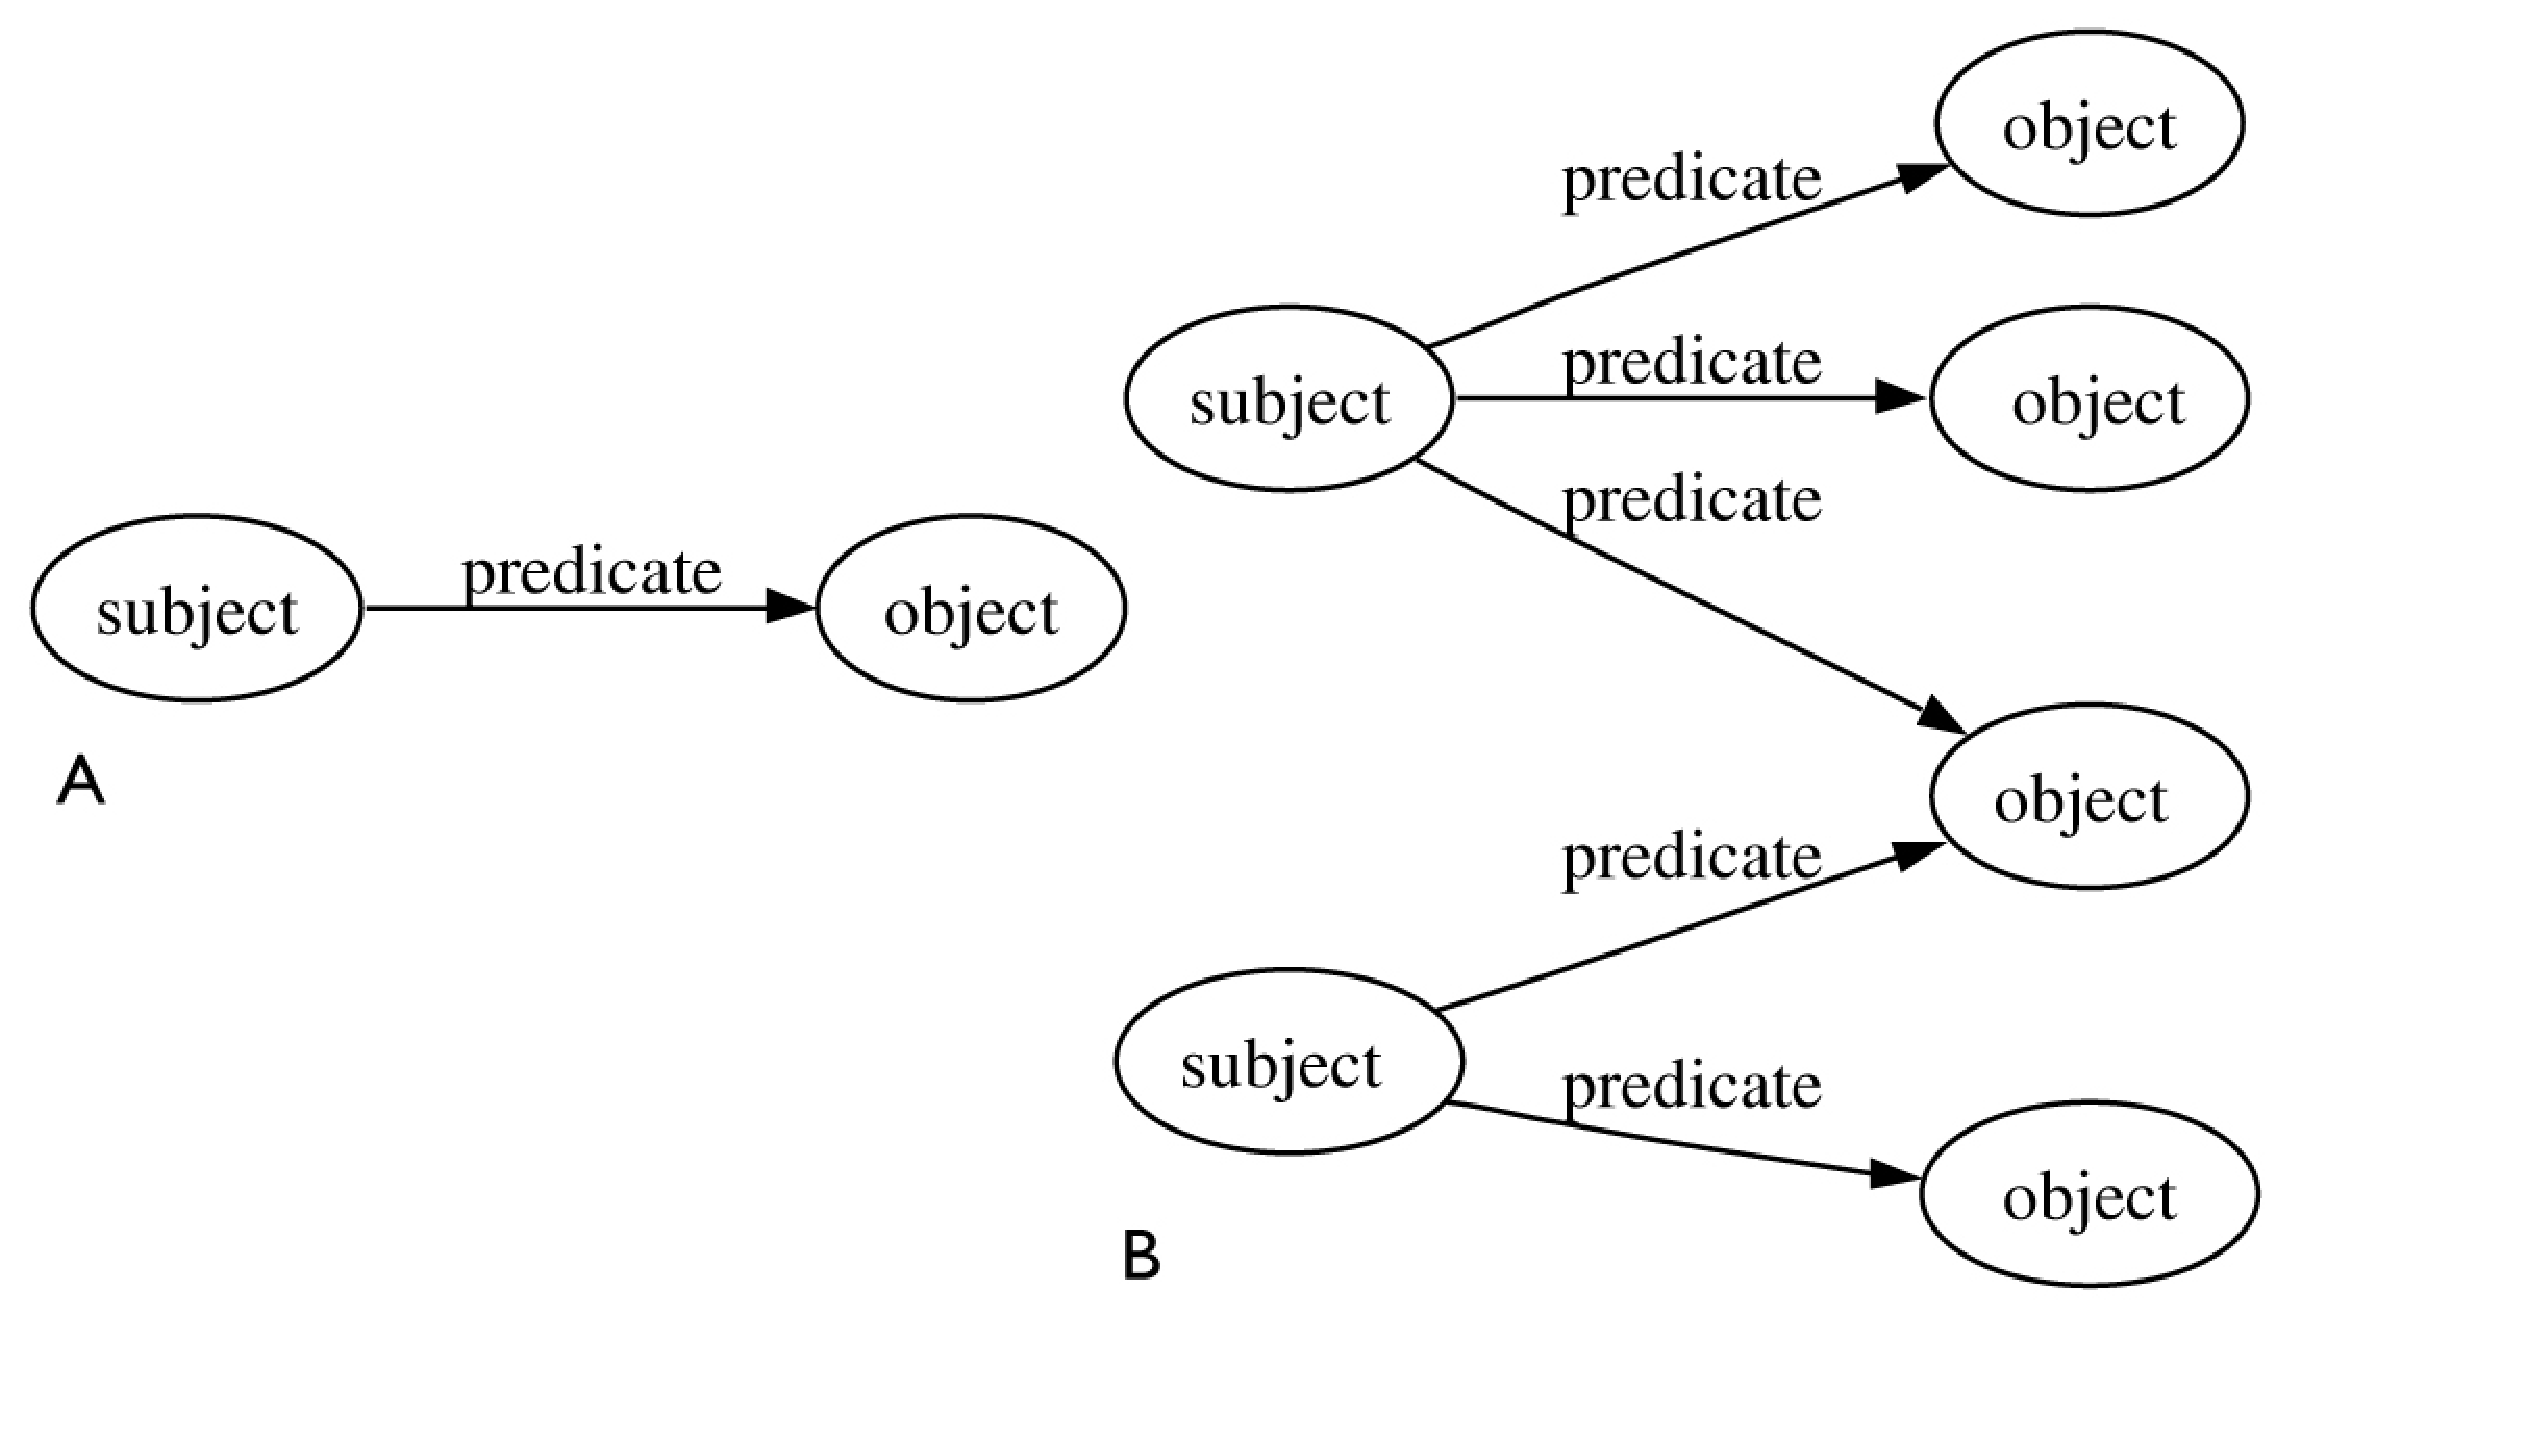
\includegraphics[width=160mm]{./images/rdf_sample.eps}
 		\caption{RDFの例}
 		\label{fig:rdf_triple}
 	\end{center}
\end{figure}

\section{SPARQLクエリ言語}
\label{knowlegde:sparql}

RDFに対するSPARQLクエリ言語の構文とセマンティクスを定義している。
SPARQLは、データがRDFそのものとして保存されているか、ミドルウェアを通してRDFとして見えるのかにかかわらず、
さまざまなデータ情報源にまたがるクエリを表わすために使用できる。
SPARQLには、必須および任意のグラフ・パターンをその論理積と論理和とともに問い合わせる性能が含まれている。
SPARQLは、ソースRDFグラフによる集約、サブクエリ、否定、式による値の作成、拡張可能な値テストやクエリの制約もサポートする。
SPARQLクエリの結果は、結果集合またはRDFグラフでありえる。
\footnote{http://www.asahi-net.or.jp/~ax2s-kmtn/internet/rdf/REC-sparql11-query-20130321}

以下は、SPARQLの例である。図\ref{sparql_sample1}がRDFグラフ\ref{rdf_sample1}のためのクエリであり、そのクエリ結果が表\ref{table:sample_sparql_result}となる。

\begin{figure}[h!]
	\begin{center}
		\lstinputlisting{./queries/sample_rdf.ttl}
		\caption{RDFサンプル}
		\label{rdf_sample1}
	\end{center}
\end{figure}

\begin{figure}[h!]
	\begin{center}
		\lstinputlisting{./queries/sample_sparql.rq}
		\caption{SPARQLサンプル}
		\label{sparql_sample1}
	\end{center}
\end{figure}

\begin{table}[h]
	\begin{center}
	\begin{tabular}{| l | l |}
		\hline
		\textbf{name} & \textbf{mbox} \\
		\hline
		"Johnny Lee Outlaw" & <mailto:jlow@example.com> \\
		\hline
		"Peter Goodguy" & <mailto:peter@example.org> \\
		\hline
	\end{tabular}
	\caption{クエリ結果}
	\label{table:sample_sparql_result}
	\end{center}
\end{table}
	
\section{Apache JenaとTDB}
\label{knowlegde:jena}

Apache Jenaとは、RDF形式のデータを処理するアプリケーションを構築するためのJavaライブラリである。
RDF用のクエリ言語SPARQLのサポートも提供される。

TDBはApache Jenaのコンポーネントの1つであるRDFストレージでり、RDFを操作するためのAPIやSPARQLエンジン、RDF用データベースである。
TDBには、各種コマンドラインツール、SPARQLサーバーなどで構成され、JenaのAPIから扱うことが出来る。RDFデータに対する推論ルールを設定することも可能である。
TDBは軽量でシンプルなRDFストレージであるが、データの挿入及び検索のパフォーマンスが比較的高く、扱いやすいRDFストレージである。

